\documentclass[11pt]{article}
\usepackage[margin=1in]{geometry}
\usepackage{amsmath,amssymb,amsthm}

\usepackage{graphicx} 
\usepackage{algorithm}               

\usepackage{algorithmic}             

\usepackage{multirow}              

\usepackage{amsmath}
\usepackage{mathtools}
\usepackage{bbm}

\usepackage{xcolor} 
\usepackage{tikz}
\usetikzlibrary{positioning}
\newdimen\nodeDist
\nodeDist=35mm


\DeclareMathOperator*{\argmin}{argmin}         

\renewcommand{\algorithmicrequire}{\textbf{Input:}}   

\renewcommand{\algorithmicensure}{\textbf{Output:}}  

\usepackage{graphics} 

\usepackage{graphicx} 

\usepackage{epsfig} 


%\usepackage{diagbox}
%\usepackage[framed,numbered]{mcode}
%\usepackage{listings}
%\lstset{language=Matlab}
%\lstset{breaklines}
%\lstset{extendedchars=false}
%
%\newcommand{\eps}{\epsilon}
%\newcommand{\inprod}[1]{\left\langle #1 \right\rangle}
%\newcommand{\R}{\mathbb{R}}

\newcommand{\handout}[6]{
  \noindent
  \begin{center}
  \framebox{
    \vbox{
      \hbox to 5.78in { {\bf CS 391L: Machine Learning} \hfill #2 }
      \vspace{4mm}
      \hbox to 5.78in { {\Large \hfill #5  \hfill} }
      \vspace{2mm}
      \hbox to 5.78in { {\em #3 \hfill #4} }
      \vspace{2mm}
      \hbox to 5.78in { {\em #6 \hfill } }
    }
  }
  \end{center}
  \vspace*{4mm}
}

\newcommand{\lecture}[5]{\handout{#1}{#2}{#3}{}{Homework
    1 - Theory - Solutions}{Keywords: Boolean functions, mistake bounds, PAC learning}}

\newtheorem{theorem}{Theorem}
\newtheorem{corollary}[theorem]{Corollary}
\newtheorem{lemma}[theorem]{Lemma}
\newtheorem{observation}[theorem]{Observation}
\newtheorem{proposition}[theorem]{Proposition}
\newtheorem{definition}[theorem]{Definition}
\newtheorem{claim}[theorem]{Claim}
\newtheorem{fact}[theorem]{Fact}
\newtheorem{assumption}[theorem]{Assumption}

\DeclareMathOperator{\pr}{\mathbb{P}}
\DeclareMathOperator{\ex}{\mathbb{E}}
\DeclareMathOperator{\ind}{\mathbbm{1}}
\DeclareMathOperator{\sgn}{sign}
\DeclareMathOperator{\err}{err}
\newcommand{\R}{\mathbb{R}}

\begin{document}

\lecture{NUMBER --- DATE, 2018}{\bf Fall 2020}{Lecture: Prof.\ Adam Klivans}{}


%{\bf Note:} Please typeset your answer (\LaTeX \ recommended) and upload it on Canvas. 
\begin{enumerate}



%	(1 point)
\item Since $f, g$ are $\{-1, 1\}$-valued, $f(x)g(x)$ is $+1$ whenever $f(x) = g(x)$ and $-1$ whenever $f(x) \neq g(x)$. Thus we can write \begin{align*} \ex_{x \sim D}[f(x)g(x)] &= (+1)\pr_{x \sim D}[f(x) = g(x)] + (-1)\pr_{x \sim D}[f(x) \neq g(x)] \\
&= 1 - 2\pr_{x \sim D}[f(x) \neq g(x)], \end{align*} using the fact that $\pr_{x \sim D}[f(x) = g(x)] = 1 - \pr_{x \sim D}[f(x) \neq g(x)]$. Rearranging the above equation proves the result.

Notice that we did not need any properties from the domain or the distribution at all for this proof, just that $f, g$ be $\{-1, 1\}$-valued. Thus the statement holds for arbitrary domains.

\item 
	We can write the decision tree as a polynomial by decomposing it in terms of its root-to-leaf paths. Consider an example path where we move along $x_1 = 1$ at the root $x_1$, along $x_3 = -1$ at $x_3$, along $x_8 = 1$ at $x_8$, and then output $-1$; in other words, if $x_1 = 1$, $x_3 = -1$, and $x_8 = 1$, output $-1$. We can represent this by the following term: \[ \left(\frac{1 + x_1}{2}\right) \left(\frac{1 - x_3}{2}\right) \left(\frac{1 + x_8}{2}\right) (-1) \] Clearly this is nonzero if $x_1 = 1, x_3 = -1, x_8 = 1$, in which case it evaluates to $-1$. In this way we can represent any path by a polynomial term. We can now write the whole decision tree $f$ by summing the terms for each of the $t$ root-to-leaf paths. Since any assignment of values to $x_1, \dots, x_n$ will follow exactly one of the root-to-leaf paths, exactly one of the corresponding terms will be nonzero, and the overall sum will be $+1$ or $-1$ according to the value at the leaf. Thus we obtain a polynomial $p$ such that $f(x) = p(x)$ for all $x \in \{-1, 1\}^n$.


\item Overall accuracy is $74\%$. The decision tree is shown below:

\begin{center}
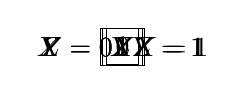
\begin{tikzpicture}[
    node/.style={%
      draw,
      rectangle,
    },
  ]

    \node [node] (A) {$Z$};
    \path (A) ++(-135:0.8\nodeDist) node [node] (B) {$Y$};
    \path (A) ++(-45:0.8\nodeDist) node [node] (C) {$X$};
    \path (C) ++(-125:0.8\nodeDist) node [node] (D) {$1$};
    \path (C) ++(-55:0.8\nodeDist) node [node] (E) {$1$};
    \path (B) ++(-125:0.8\nodeDist) node [node] (F) {$0$};
    \path (B) ++(-55:0.8\nodeDist) node [node] (G) {$1$};

    \draw (A) -- (B) node [left,pos=0.25] {$Z=0$}(A);
    \draw (A) -- (C) node [right,pos=0.25] {$Z=1$}(A);
    \draw (C) -- (D) node [left,pos=0.25] {$X=0$}(A);
    \draw (C) -- (E) node [right,pos=0.25] {$X=1$}(A);
    \draw (B) -- (F) node [left,pos=0.25] {$Y=0$}(A);
    \draw (B) -- (G) node [right,pos=0.25] {$Y=1$}(A);
\end{tikzpicture}
\end{center}

The calculations are as follows:


\textbf{Root node: }
Note that the potential for all the examples is $C(Pr[Pos]) = 2 * \frac{165}{250} * \frac{85}{250} = 0.4488$.

If we choose $X$ to be the root node, then the new expected potential is $Pr[X = 0] C(Pr[Pos | X = 0]) + Pr[X = 1] C(Pr[Pos | X = 1]) = \frac{150}{250} * C(\frac{105}{150}) + \frac{100}{250} * C(\frac{60}{100}) = 0.444$

If we choose $Y$, it is $\frac{120}{250} * C(\frac{70}{120}) + \frac{130}{250} * C(\frac{95}{130}) = 0.422949$. 

If we choose $Z$ it is $\frac{120}{250} * C(\frac{60}{120}) + \frac{130}{250} * C(\frac{105}{130}) = 0.401538$.

So, $Z$ minimizes the new potential, or in other words, it maximizes the information gain which is $0.4488 - 0.401538 = 0.047262$. Thus, we should pick $Z$ to be the root node.

\textbf{Left node: } Since an example only enters the left node when $Z = 0$, we will restrict ourselves to the examples where $Z = 0$.

Note that the total potential in this case is $C(\frac{60}{120}) = 0.5$.

If we choose $X$ to be the left node, then the new expected potential is $\frac{80}{120} * C(\frac{45}{80}) + \frac{40}{120} * C(\frac{15}{40}) = 0.484375$

If we choose $Y$ to be the left node, then the new expected potential is $\frac{50}{120} * C(\frac{15}{50}) + \frac{70}{120} * C(\frac{45}{70}) = 0.442857$

Thus, choosing $Y$ minimizes the new expected potential, or maximizes the information gain which is $0.5 - 0.442857 = 0.057143$. Since in this case, we have more examples labeled negative then positive when $Y = 0$, we will output negative when $Y = 0$. Similarly, we have more examples labeled positive than negative when $Y = 1$, and so when $Y =1$, we will output positive.

\textbf{Right node:} Since an example only enters the right node when $Z = 1$, we will restrict ourselves to the examples where $Z = 1$.

Note that the total potential in this case is $C(\frac{105}{130}) = 0.31065088757$.

If we choose $X$ to be the right node, then the new expected potential is $\frac{70}{130} * C(\frac{60}{70}) + \frac{60}{130} * C(\frac{45}{60}) = 0.304945$

If we choose $Y$ to be the right node, then the new expected potential is $\frac{70}{130} * C(\frac{55}{70}) + \frac{60}{130} * C(\frac{50}{60}) = 0.309524$

Thus, choosing $X$ minimizes the new expected potential, or maximizes the information gain which is $0.31065088757 - 0.304945 = 0.00570588757$. Since in this case, we have more examples labeled positive then negative when $X = 0$, we will output positive when $X = 0$. Similarly, we have more examples labeled positive than negative when $X = 1$, and so when $X =1$, we will output positive.

Our accuracy is computed as (number of examples our decision tree labels correctly)/(total number of examples). In this case, this is $\frac{185}{250} = 0.74 = 74\%$.

\item This is actually a strictly simpler, instructive version of the axis-parallel rectangles problem from lecture. As in that problem, the algorithm is very natural: draw a large number (say $m$) of examples, and then pick the ``tightest-fitting'' threshold function. More concretely, we can arrange our training data in ascending order in terms of $x$, and then pick the largest $x$ that is labeled $-1$ as our threshold. (Another approach would be to pick the smallest $x$ that is labeled $+1$; this also works and has a nearly identical analysis.) This can be done efficiently in $O(m)$ time by going through all $m$ points. (Aside: we cannot use binary search since the points don't arrive in sorted order.) What remains is the analysis of how large $m$ needs to be in order to be have high confidence that our output has low error.

To do this, suppose $h_\theta$, for some $\theta \in \R$, is the true threshold function that is labeling the data. Suppose that the threshold we obtain (by picking the largest $x$ labeled $-1$ in our dataset) is $\hat{\theta}$. Notice that we will necessarily have $\hat{\theta} \leq \theta$, and the only area where $h_{\hat{\theta}}$ differs from the true $h_\theta$ is the interval $[\hat{\theta}, \theta]$. This is where our classifier errs, and the error is precisely the probability mass of this interval.

Define $B$ to be the interval immediately to the left of $\theta$ that has probability mass $\epsilon$. Observe that if we get even one training point in $B$, then we are guaranteed that $[\hat{\theta}, \theta]$ lies within $B$, and so our error will be at most $\epsilon$. Thus, our bad event is that none of our $m$ training points fall in $B$. The probability of this happening is $(1 - \epsilon)^m \leq e^{- \epsilon m}$ (using the fact that $1 + x \leq e^x$ for all $x$), which can be made at most $\delta$ by picking $m = \frac{1}{\epsilon} \log \frac{1}{\delta}$. This completes the analysis.


% Auto-generated using Mathcha! Nice :) Then lightly edited
\tikzset{every picture/.style={line width=0.75pt}} %set default line width to 0.75pt        

\begin{center}
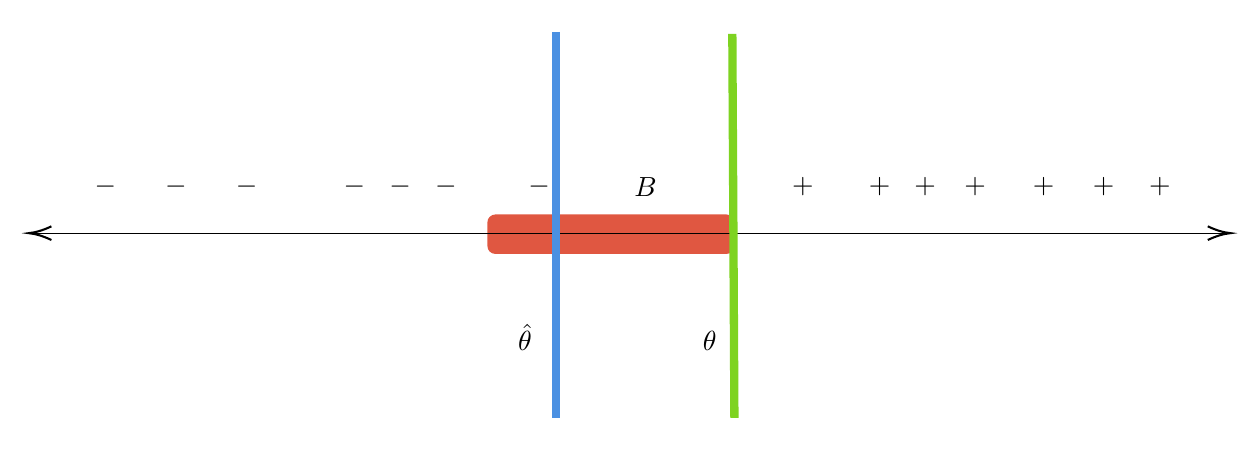
\begin{tikzpicture}[x=0.75pt,y=0.75pt,yscale=-1,xscale=1]
%uncomment if require: \path (0,300); %set diagram left start at 0, and has height of 300

%Rounded Rect [id:dp8007893628810216] 
\draw  [draw opacity=0][fill={rgb, 255:red, 224; green, 87; blue, 65 }  ,fill opacity=1 ] (268.5,186.8) .. controls (268.5,184.7) and (270.2,183) .. (272.3,183) -- (383.7,183) .. controls (385.8,183) and (387.5,184.7) .. (387.5,186.8) -- (387.5,198.2) .. controls (387.5,200.3) and (385.8,202) .. (383.7,202) -- (272.3,202) .. controls (270.2,202) and (268.5,200.3) .. (268.5,198.2) -- cycle ;
%Straight Lines [id:da05201696079188789] 
\draw    (49.5,192) -- (624.5,192) ;
\draw [shift={(626.5,192)}, rotate = 180] [color={rgb, 255:red, 0; green, 0; blue, 0 }  ][line width=0.75]    (10.93,-3.29) .. controls (6.95,-1.4) and (3.31,-0.3) .. (0,0) .. controls (3.31,0.3) and (6.95,1.4) .. (10.93,3.29)   ;
\draw [shift={(47.5,192)}, rotate = 0] [color={rgb, 255:red, 0; green, 0; blue, 0 }  ][line width=0.75]    (10.93,-3.29) .. controls (6.95,-1.4) and (3.31,-0.3) .. (0,0) .. controls (3.31,0.3) and (6.95,1.4) .. (10.93,3.29)   ;
%Straight Lines [id:da415344239216764] 
\draw [color={rgb, 255:red, 74; green, 144; blue, 226 }  ,draw opacity=1 ][line width=3]    (301.5,95) -- (301.5,281) ;
%Straight Lines [id:da9378945364065577] 
\draw [color={rgb, 255:red, 126; green, 211; blue, 33 }  ,draw opacity=1 ][line width=3]    (386.5,96) -- (387.5,281) ;

% Text Node
\draw (282,234.4) node [anchor=north west][inner sep=0.75pt]    {$\hat{\theta }$};
% Text Node
\draw (371,237.8) node [anchor=north west][inner sep=0.75pt]    {$\theta $};
% Text Node
\draw (78,164) node [anchor=north west][inner sep=0.75pt]    {$-$};
% Text Node
\draw (198,164) node [anchor=north west][inner sep=0.75pt]    {$-$};
% Text Node
\draw (112,164) node [anchor=north west][inner sep=0.75pt]    {$-$};
% Text Node
\draw (146,164) node [anchor=north west][inner sep=0.75pt]    {$-$};
% Text Node
\draw (220,164) node [anchor=north west][inner sep=0.75pt]    {$-$};
% Text Node
\draw (242,164) node [anchor=north west][inner sep=0.75pt]    {$-$};
% Text Node
\draw (287,164) node [anchor=north west][inner sep=0.75pt]    {$-$};
% Text Node
\draw (414,164) node [anchor=north west][inner sep=0.75pt]    {$+$};
% Text Node
\draw (451,164) node [anchor=north west][inner sep=0.75pt]    {$+$};
% Text Node
\draw (473,164) node [anchor=north west][inner sep=0.75pt]    {$+$};
% Text Node
\draw (497,164) node [anchor=north west][inner sep=0.75pt]    {$+$};
% Text Node
\draw (530,164) node [anchor=north west][inner sep=0.75pt]    {$+$};
% Text Node
\draw (559,164) node [anchor=north west][inner sep=0.75pt]    {$+$};
% Text Node
\draw (586,164) node [anchor=north west][inner sep=0.75pt]    {$+$};
% Text Node
\draw (338,164) node [anchor=north west][inner sep=0.75pt]    {$B$};
\end{tikzpicture}
\end{center}



\item
  \begin{enumerate}
  	\item If $\err(h) > \epsilon$, then the probability that $h$ labels a single
  	randomly drawn example correctly is less than $1-\epsilon$. The probability of getting $k$ independent examples right is less than $(1 - \epsilon)^k \leq e^{-\epsilon k}$ (using the fact that $1 + x \leq e^x$ for all $x$). By picking $k = \frac{1}{\epsilon}\log \frac{1}{\delta'}$, this is at most $\delta'$ (which, as we'll see, will be picked based on our final desired $\delta$).
  	\item Since $A$ has a mistake bound of $t$, and it only updates when it makes a mistake, it can go through at most $t$ hypotheses. This means that if we view our examples as consisting of $t + 1$ blocks of size $k$, then we must have a block where we make no mistakes.
  	\item The event $E_i$ occurs when we output $h_i$ such that $\err(h_i) > \epsilon$. Based on our steps so far, the most natural idea for when we decide to stop and output $h_i$ is to do so when $h_i$ has gotten its block of $k$ examples right.\footnote{Important pedagogical note: when we talk of the event $E_i$, we are saying something about the \emph{examples}, not the hypothesis per se ---  we are saying that the $i$th block is misleading in the technical sense that all $k$ examples happen to fall into $h_i$'s ``good area''. That is, the function is fixed, and it is the examples that are random. It's important to understand this fact in this kind of analysis. If you like, the sample space consists of realizations of our random draws of examples from $D$.} So the hypothesis our PAC learner eventually outputs will be one of the $h_i$ that $A$ goes through. The PAC learner's failure event is precisely that it outputs a hypothesis with error greater than $\epsilon$, and is thus described by $E = \cup_i E_i$. Here the union is taken over all the blocks we go through, which number at most $t + 1$.
  	\item The overall PAC learner is as follows: \begin{itemize}
  		\item The learner first draws $(t+1)k$ random examples from $D$ and arranges them into $t + 1$ blocks of size $k$.
  		\item At the start of each block, we will assume that algorithm $A$, with its current state/hypothesis $h_i$, satisfies $\err(h_i) \leq \epsilon$, and will use the examples in the block to test if this is indeed the case.  Given a block of examples, the learner feeds examples one by one to $A$.  If $A$ makes a mistake labeling one of the examples in a block, we move on to the next block. If it does not, we stop and output $h_i$.
  	\end{itemize} As we saw, the failure event of this algorithm is $E = \cup_i E_i$, and we want to ensure that $\pr[E] \leq \delta$. By the union bound, we can say that $\pr[E] \leq \sum_i \pr[E_i]$. Recall that we picked $k$ such that $\pr[E_i] \leq \delta'$. Since there are at most $t + 1$ events $E_i$, picking $\delta' = \delta/(t+1)$, we have $\pr[E] \leq (t+1)\delta' \leq \delta$, as desired. This proves the correctness of our PAC learner. The total number of examples used is $(t+1)k = \frac{t+1}{\epsilon} \log \frac{t+1}{\delta}$.
  \end{enumerate}

\end{enumerate}


\end{document}

